% !TeX root = ../main.tex

\chapter{eFF 势函数计算在申威处理器上的优化方法}

\section{从核通信规约}
无论是内层循环并行,副本归约还是内端更新方法中,都需要进行对从核计算中的受力信息的累加,以此消除数据依赖的问题。为了保证整个从核计算的性能发挥,这里设计了一个高效的从核核组内的通信模式。由于每个粒子在从核内进行累加的变量占用的 LDM 空间相对有限,所以这里同样从核 LDM 内开辟了一份临时空间用于进行变量的累加。这种通信方式只涉及从核LDM 的使用,并不进行主核计算和占用主存空间,因此也避免了访存带来的额外开销。

对于从核通信归约,首先需要保证所有参与该轮计算的从核完成对当前粒子受力信息的计算,该部分结果保存在所有从核所在的LDM 中。申威处理器从核间通信采用的是寄存器方式进行不同从核间的通信,这里采用一种多层数据归约的方法完成最终结果的累加,每次按从核序号进行当前一半从核结果的归约,对于 64 个从核来说总共只需要 6 轮累加即可得到最终的计算结果。首先进行行内从核得累加,将每行结果归约到行首第一个从核内,第一轮将行内所有奇数编号从核向前一个从核得临时空间内写入结果,在结果写入完成后,开始进行偶数编号从核的累加,该轮归约主要针对行内第2,6 号从核,在发送结果之前,先将从核自身的结果累加到临时空间,再将累加后的结果分别向第 0,4 号从核进行发送。此时在行内的第 0 号从核保存行内第 0 到第 3 个从核累加后的结果,第 4 号从核保存第 4 到第 7 号从核得结果,再将第 4 号从核结果发送给第 0 号从核即可得到本行结果的累加,结果保存在对应从核LDM 中。行内归约完成后,所有结果都保存在核组内第一列的从核中,此时只需要按照行内归约的方法就能将第一列从核结果归约到第0 号从核中,在全部结果归约完毕后,只需要由第0 号从核将结果写回就能完成此轮的计算。

仅仅给出核组内多层数据归约的通信方法还不能完全解决整个核组内局部写回变量的累加。由于多个从核会同时进行从核数据通信,就不可避免地由于归约次序不一致,导致累加结果产生错误。因为同一个从核每次只能完成来自一个从核数据的接收,如果此时一个从核需要完成来自多轮不同从核数据的累加,由于不同从核执行速度的差异,会导致一个从核会在同一轮收到来自多个从核的结果。为了解决这种不同从核执行次序的问题,这里采取了对核组内进行从核同步的方案,并且为了保证从核同步的性能,只采用点对点的方式进行从核同步,在每次从核发送数据之前,先于所要接收数据的从核进行点对点的同步,之后再完成当前从核数据的发送。例如在从奇数号从核向偶数号从核发送数据之前,先进行双方从核间的同步,再将偶数号从核的数据发送至奇数号从核得临时空间,以此类推,直到完成所有从核数据的归约。

 \begin{figure}[h]
  \centering
  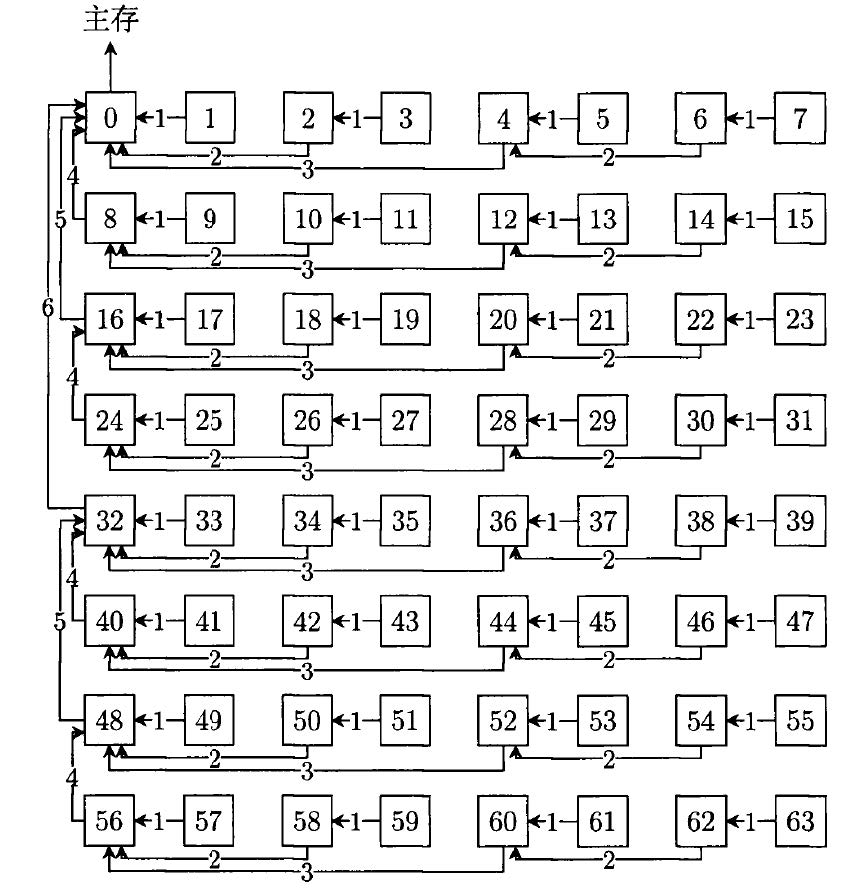
\includegraphics[width=0.7\textwidth]{4_1.jpg}
  \caption{从核通信规约}
  \label{fig:badge}
\end{figure}

\section{从核访存优化}
本节主要介绍如何通过优化读写数据的方法来减少访存在带宽上的开销。从核阵列负责了绝大部分势函数及受力的计算,也就不可避免地需要对主存进行大量频繁地读写操作。在从核还未进行计算时,会从主存读取当前时间步所需要计算粒子的数据信息,包括位置坐标,类型,带电量等,而在每个时间步内从核阵列又会多次进行访存操作。除此之外,由于指令集的要求,对于从核阵列的数据读写,要先从LDM 局存读入对应的寄存器,再将相应的数据写回到内存地址空间。由于分子动力学应用普遍存在着计算密集的特点,而从核阵列自身并没有数据cache 的设计,也就意味着无法对频繁访问的粒子信息进行高效的重用,而对于整个从核阵列仅有 30GB/s 的带宽,从核同时进行访问无疑会造成激烈的带宽竞争,使得在从核计算时访存成为阻碍性能提升的瓶颈。这里我们选择 DMA访问方式与预取频繁被调用数据的方法来降低访存的开销。

\subsection{采用DMA方法降低访存开销}
从核在进行访存操作时,最简单的方法是直接访问主存地址进行数据读写,这种方法被称为gld/gst,但由于从核没有设计数据cache 的原因,这种方法在多次访存时开销较大。对于申威异构处理器还可利用DMA 的方式进行从核访存操作,通过DMA\_GET 访存接口,便可以在主存空间内连续读取数据到从核LDM指定地址,通过DMA\_PUT 接口由从核向主存发起写操作请求。由于DMA 操作可以异步执行,所以在从核发出DMA 请求后仍可以继续完成其他操作而无序进行等待。利用DMA 进行于数据读写的方式有两种,一是直接通过DMA 原语进行 DMA 请求,另外一种是通过申威平台提供的 athread 函数库进行 DMA 请求。在之前的实验分析中我们了解到由于发起DMA 请求需要进行初始化过程,而在单次传输较小的数据块时性能与 gld/gst 方式无异,只有在传输数据块大小至少为 128 字节的时候,带宽才趋近于饱和,性能也相比直接访存有着较大的提升。

在LAMMPS 势函数的计算中,主要通过两层迭代实现对粒子间受力的计算,其中外层循环的粒子访问是连续的,其中包括粒子位置坐标,自旋类型,带电量等数据信息,并且对于每个粒子的邻接表访问也同样是连续的,这样就使得采用 DMA 方式访存的优势变得更加显著,在进行粒子信息读取的过程中,由于不同粒子的存储是离散的,但对于粒子的相对位置是固定的。所以这里选择不同粒子信息分别发起DMA 请求操作,这里包括多个粒子的数据块要大于128 字节,所以能够充分利用访存带宽,同时减少从核得访存频率,进一步提高访存效率。


\subsection{采用预取暂存的方式}
为了进一步提高访存效率,充分利用有限的访存带宽,这里我们设计了一种类似于通用处理器的缓存预取策略。在进行从核计算之前,将需要参与计算的数据手动预取到从核LDM 中。在实现预取策略之前,首先分析所应当获得的数据基本特性。对于从核来说,由于并没有数据cache 的设计,此时就需要充分利用与其性能相近的LDM 进行数据存储。首先,所访问的数据可能局部性特性并不明显,但通过手动分析发现其在整个时间步计算内频繁地被调用和访问。当这部分数据开始参与计算之前,不需要进行访问主存,而只需要从当前LDM 空间获取即可,这样不仅能提高访存性能,而且由于从核阵列访存带宽有限,又能解决带宽不足的问题。通过对计算热点和算法的分析,这里选用在计算中参与次数最多的数据暂存在LDM 中,以提高访存性能。其次,数据自身的体积也是需要考虑的问题,对于仅有几千个粒子的模拟体系,带有双精度的粒子位置坐标等信息的存储就要消耗几百 KB 的空间,而对于只有 64KB 存储空间的 LDM 来说,这无疑是不可接受的,所以对于有限的存储空间必须选择体积较小的计算信息进行暂存,并通过实验分析合适的数据量大小,保证不超过LDM 局存的最大空间。

从核进行热点函数计算之前,先通过一轮DMA 操作分别将所要暂存的粒子数据发送到从核LDM 中,其中包括计算标志位和参数等信息。对于已经暂存到局存内的数据,在访问时不需要再从主存进行访问,只要从LDM 进行读写,而对于大量计算时调用的粒子结构数据,则仍然在计算时利用DMA 读取,经过统计,对于每个从核在每个时间步内的计算,每次大约读取 17KB 的数据进行暂存。而在当前时间步计算后,只有对部分暂存数据进行了改写,并对这部分数据进行写回操作,通过预取数据暂存的方法,可以进一步保证访存效率,提升整体计算性能。

\section{单端更新并行方法}
在对LAMMPS 势函数计算进行任务划分时,其关键是对内外两层粒子的迭代进行划分,并根据所在循环的粒子规模,选择合适的划分粒度,保证从核的负载均衡和计算的并行性。在任务划分的基础上,针对产生的从核数据依赖问题,给出不同的依赖解决办法。在通过从核间通信与访存优化后,如何继续提高计算并行的方案,则是我们更加需要关心的问题,其中要解决的核心问题是如何利用有限的硬件存储资源,消除任务划分时棘手的数据依赖问题,在之前内层的循环并行方法中,之所以没有对两层循环同时划分,是因为在进行中心粒子与邻居粒子的受力计算时,同一个粒子可能会同时作为多个粒子的邻居而被划分到不同从核内,此时就会导致同一个粒子的受力信息会被不同从核同时更新而在写回主存时产生写写依赖的问题。之前我们提出了一种解决办法,就是通过副本归约而方案,将每个粒子的受力信息以临时数据的形式保存在从核LDM 中,再通过指定的从核在当前时间步计算结束后进行临时数据的累加并写回主存。这种方案虽然可以解决数据依赖的问题,但是同时又会提出新的困难,就是要在本就空间受限的局存LDM 中再开辟出一份临时空间作为数据存储,并且由于同时还需要在 LDM 中分配空间给软件 cache 的设计和频繁调用数据的预取和暂存,这种代价对于大规模体系的计算中,无疑是不可接受的。除了副本归约的方案外,解决依赖问题还可以使用从核的原子更新指令,但由于这种指令限制较大,且更新周期较长,对于大规模计算也不是很合适。

 \begin{figure}[h]
  \centering
  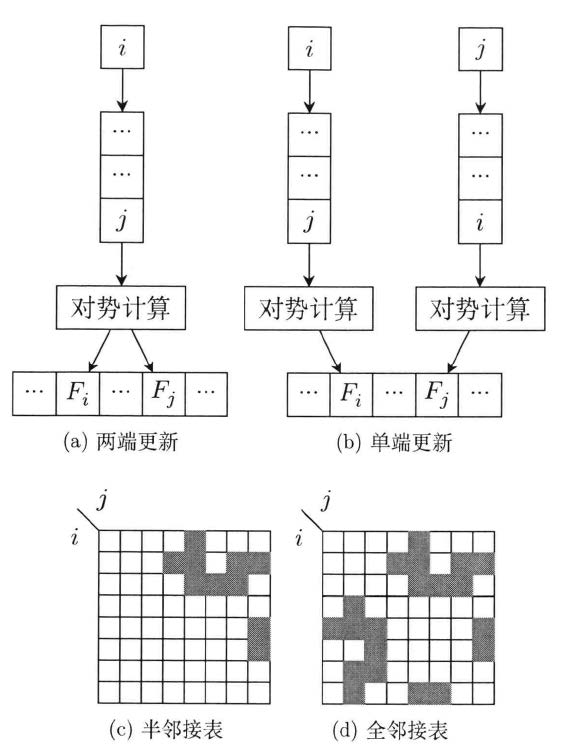
\includegraphics[width=0.5\textwidth]{4_2.jpg}
  \caption{单端更新并行算法}
  \label{fig:badge}
\end{figure}

在进行LAMMPS 势函数的计算时,对邻居粒子受力信息的更新是与粒子自身同时进行的,这是由于分子动力学对牛顿第三定律的引入所导致的。牛顿第三定律指出,粒子间的受力是以相互作用力的形式体现的,其受力与反作用力是一种大小相等,方向相反的状态,也就是说在进行受力更新时,只需要计算两个粒子两个粒子在这个时间步的作用力,再以相反的数值累加到粒子的总受力上即可。这也使得粒子对间的计算量能够下降一半,提高计算效率。但对于计算的并行这却是灾难的来源,这种计算本身引入了粒子数据依赖,为了解决这个问题,这里选择不采用牛顿第三定律的做法,而是对粒子对间的计算分为两次进行。这样考虑一方面是因为对于申威众核平台上并行效率与访存开销是影响性能的关键。另一方面也是因为对于eFF 势函数计算量的增加并非不可接受,这样用计算量来换取访存性能与并行效率的方案,实际上对整体性能仍然是一个很多的提升。这里我们给出 LAMMPS 中 eFF 势函数的计算开销表示:

其中 𝑇𝑒𝐹 𝐹 表示完成势函数过程花费的总时间,𝑇𝑟𝑖/𝑗 为读取中心粒子和邻居粒子的时间,𝑇𝑤𝑖/𝑗 为将粒子写回主存的时间,𝑇𝑐𝑢𝑙 为 eFF 势函数计算花费的时间。其中在进行缓存优化后,𝑇𝑟𝑗 主要由缓存读取开销决定。既然是将邻居粒子计算单独进行,所以这里需要关注的是𝑇𝑟𝑗 , 𝑇𝑤𝑗 与𝑇𝑐𝑢𝑙 之间的关系,并且由于𝑇𝑟𝑗开销较小,所以如何减小 𝑇𝑤𝑗 就成为了优化的重心。

通过对算法的修改,我们选择在进行<i,j> 粒子对的计算后,只进行对i 粒子受力信息的更新,同理在 <j,i> 粒子对完成后,也只更新 j 粒子的受力信息,这样就能够保证在同一个时间步内不会存在多个从核对同一个粒子更新受力而产生的数据依赖问题。另外为了适应粒子计算的变化,这里需要也对邻接表进行相应的修改,在邻接表内保存着体系中当前时间步每个粒子以及邻居粒子的序号,并通过进一步对粒子间距离与截断半径的比较,进行下一步粒子间的计算过程。对于采用牛顿第三定律的势函数计算来讲,由于每次计算会同时更新两个粒子的受力信息,邻接表是以半邻接的形式表示,此时只需在一次计算中同时更新两个粒子的受力即可。对于单端更新并行方法,每次计算只会有一个粒子的受力被更新,也就是说在邻接表内<i,j> 与<j,i> 粒子对的位置需要同时被标记,这种邻接表称为全邻接表。在具体表示中,半邻接表相当于矩阵中的一个上三角或下三角矩阵,全邻接表则是将这个矩阵对称到另一个三角区域。

除了进行受力更新之外,能量累加的计算也同样需要被考虑,当前计算会同时计算 <i,j> 和 <j,i> 粒子对,在进行总能量更新时,需要将能量的累加转换为原来的一半,否则在进行压强和温度的统计中会发生结果的偏差,在采用单端更新方法后,原本的 eFF 势函数计算可表示为:

可以看出相对于原来的计算框架,这里增加了 𝑇𝑟𝑗 和 𝑇𝑐𝑢𝑙,但却节省了 𝑇𝑤𝑗写回粒子数据的时间,由于𝑇𝑟𝑗 主要从缓存中读数据,其开销相对较小,并且eFF计算量并不算大,所以在对于 𝑇𝑟𝑗 􀀁𝑇𝑐𝑢𝑙 与 𝑇𝑤𝑗 的权衡时,整体性能能够有一个明显的提升。

\section{软件cache优化方法}
在进行LAMMPS 势函数计算时,对于粒子的访问是通过邻接表索引来进行的。采用邻接表方式进行访问自身是以一种离散的方式进行的,每个粒子及其邻居粒子都在邻接表中以非连续的序号进行排列,通过对 eFF 势函数计算进行大量的分析和总结后,这些通过邻接表访问的粒子及其邻居粒子仍存在较高的局部性,例如在一个三维的体系中,一个粒子的邻居集合与其附近粒子的邻居集合间绝大部分是重叠的。就是说进行势函数计算时粒子是以顺序的方式进行排列的,在一段时间内会多次访问这部分粒子及其相关数据信息,这也说明了在eFF 计算中存在着较强的时间局部性(Temporal Locality)和空间局部性(Spatial Locality)特征。这些局部性特征的存在,使得分子动力学计算能够在 X86 等含有多级Cache 的处理器上拥有良好的访存性能。对于申威处理器来说,负责主要计算任务的从核阵列没有采用数据 Cache 这种结构设计,也就从一定程度上失去了利用程序局部性来提高访存性能的机会。为了捕获程序局部性这种性能优化的特征,这里设计了以从核 LDM 为基础的软件 Cache 的存储结构。Cache 的本质只不过是在主存和寄存器之间添加了一个额外存储空间。使整个存储层次有更好的容量与延迟的匹配关系,以这个角度来看,从核LDM 与Cache 有着相类似的存储特性。相对于主存,有着更低的延迟,相对于寄存器,有着更大的空间。唯一不同的是,传统Cache 的设计是透明的,而从核LDM 则需要手动管理。

 \begin{figure}[h]
  \centering
  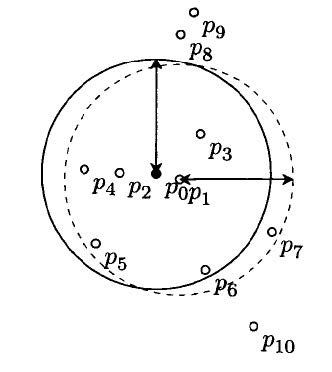
\includegraphics[width=0.5\textwidth]{4_3.jpg}
  \caption{邻居粒子具有局部性}
  \label{fig:badge}
\end{figure}

在一个任务与计算的执行过程中,对于任何一条存储指令和访存指令在到达目标寄存器之前,都可能出现Cache Hit 和Cache Miss 两种情况,这样就很难准确计算在这个计算过程中每次独立的存储器访问时间,所以对统计访存性能的关键就落到了计算存储器平均访问时间 AMAT(Average Memory Access Time),这里给出 AMAT 公式如下:

其中Hit time 是处理器访问数据单元在Cache 中命中所花费的时间,主要为查找数据和加载到寄存器中的用时。Miss Rate 是发生 Cache Miss 的比例,Miss Penalty 是发生不命中行为后在更低级存储单元内加载数据的时间。

接下来是对于缓存组成方式的选择,常见的有全相联,多路组相联和直接映射三种方式,其中多路组相联有可以进行多种选择。组相联映射是将Cache 分为多个组,,每个主存页可以映射到每个组中选定的位置,全相联和直接映射只不过是两个特例。虽然根据平台和缓存层次不同,当前多数通用平台 CPU 缓存的设计都采用多路组相联的方式,这样既兼顾了直接映射的性能,又限制了过高的设计复杂度。但对于在从核LDM 上的软件Cache 无法直接套用这个想法,最主要的原因是设计软件 Cache 而非由硬件完成操作的代价开销不可忽略。在实际对比仅有两路组相联和直接映射对比的情况中,直接映射的整体性能也要更优。这是因为在组相联的设计中带有多层判断语句,使流水线性能大幅下降,虽然能保证更高的命中率,但对于命中时间则有较大影响,在进行对个角度的平衡和实验后,这里选择了直接映射作为缓存块的组织方式。

地址转换是从核软件 Cache 设计的关键,通过地址转换来判断当前访问的地址数据在Cache 中是否命中,若命中直接从Cache 中取对应的数据,若缺失则转向进行主存 DMA 操作。对于地址转换,首先将对访问的粒子序号进行拆分,分为标志位,页号和页内偏移三部分,这里通过页号的查找获取对应页号的标志位,再通过标志位之间的对照,若一致则表示数据命中,不一致则需要进行DMA 的访存操作。访存时先将对应数据放到软件 Cache 对应的页中,再进行标志位的修改,最后再根据偏移找到对应数据的具体位置并读入寄存器。在进行地址转换的简单做法是通过除法操作找到标志位,页号等信息,但由于在申威平台上除法指令是利用间接实现的,所以在性能方面考虑,这里使用位运算进行地址转换过程。

软件 Cache 的设计由于使得其访存延迟与性能无法直接媲美硬件架构下的Cache,这里通过对粒子数据进行打包的方法继续降低软件 Cache 的指令数量。首先对于 eFF 势函数的计算,包括三维双精度粒子坐标,整数粒子类型,整数自旋类型,浮点类型的波包半径,浮点类型带电量,共有5 个浮点类型,2 个整数类型,把这些数据打包成一个结构体,并在结构体后填充 16 字节用于数据对齐。对于256 字节的Cache 可以保存4 个粒子数据,在32KB 的空间内可以存放128 个 Cache 页。添加填充数据可以保证在访存时以对齐的方式读取每个 Cache页,对于申威处理器平台,从核每次只能访问对齐的数据块,并且如果设置从核以 64 字节为单位进行访存,对于非对齐的 64 字节数据则一定会拆为两个数据块分两次进行访存,极端情况下甚至在只有数个字节也会被拆为两次进行访存,这种情况会进一步提高访存代价 Miss Penalty,并占用额外的访存带宽。

\section{向量化方案}
对于分子动力学势函数计算,每次迭代都会进行多个粒子间的受力计算。这里选择利用向量化指令进一步优化 eFF 势函数计算的性能,并利用申威处理器提供的一套完整的256 位向量化指令操作。对于向量化计算,每次会对4 个不同粒子进行受力结果的计算。在利用访存优化,软件Cache 的设计及单端更新方法对访存开销进行优化后,计算部分在整个势函数中占据的比例逐渐提高,而采用向量化方法就是继续提升计算性能的方法。在进行向量化操作之前,我们需要先确定在计算中需要进行向量化的位置,如果对外层迭代进行向量化操作,由于每个粒子的邻居粒子不同,可能会导致因为粒子类型差异而采用不同计算,并且外层需要的分支较为负责,使用向量化难度较高,性能提升相对有限。所以这里选择对内层的邻居粒子进行向量化操作,从核浮点向量化长度为256 位,这里选择以四个粒子为单位进行向量化操作。

 \begin{figure}[h]
  \centering
  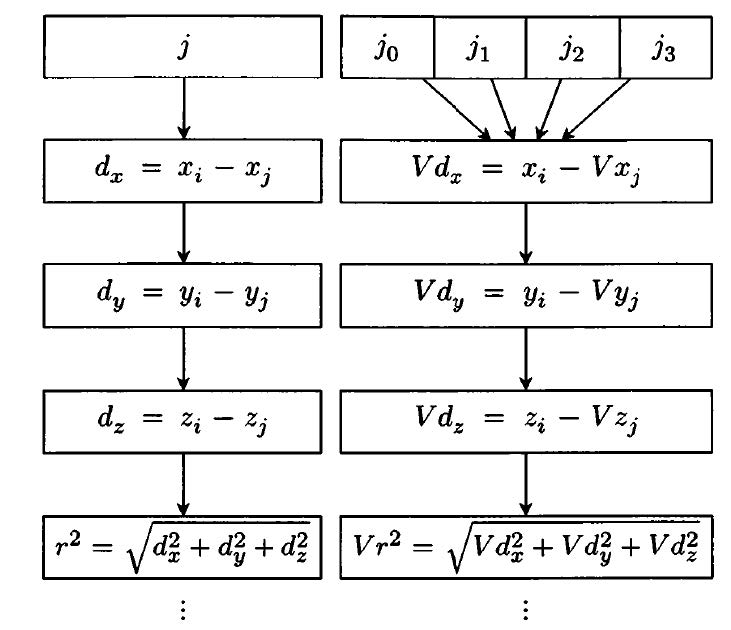
\includegraphics[width=0.5\textwidth]{4_4.jpg}
  \caption{对粒子进行向量化操作}
  \label{fig:badge}
\end{figure}

首先需要解决离散粒子数据如何读到向量结构中的问题,对于计算时的粒子信息,在计算开始之前,可能分布在不同的位置,例如在主存中还没有被调用到 Cache 中或者已经被淘汰了出来,又可能已经保存在了从核 LDM 的软件Cache 内。一般情况下,对于只在同一个存储层次内的数据可以直接依赖向量读取指令读取到向量单元内,而对于需要读取到一个向量单元内之前却分布在不同存储层次的数据,没办法直接利用向量读取指令的方法进行读取。这里通过申威平台向量混洗指令的支持来进行离散粒子的读取。操作向量混洗指令是通过对两个256 位的向量进行手动调整,通过特定操作码的分配,得到目标向量的过程。该指令的输入参数为两个源向量以及一个 8 位的控制码。在 8 位控制码中,每两位控制码为一组,共分为四组,每组控制码指示目标向量来自源向量的浮点元素位置,四组对应四个64 位数据的分配。又以每4 位控制码对应一个源向量,指向目标向量的高两位或者低两位,也就是说,在目标向量的位置上,固定有两个元素来自其中一个源向量,位置由控制码指定。

在之前的软件Cache 的设计中,每个粒子信息需要占用512 位的空间,包括三个双精度浮点坐标,一个双精度带电量和一个双精度波包半径信息,以及两个整形类型数据。由于从核向量长度是256 位,这里将每个粒子的数据拆分为两个向量进行存储,前一个保存三个坐标位置和一个带电量信息,后一个保存波包半径和两个整型信息数据,其中每个整型数据单独占用 64 位的空间,并在其余的位置填充空数据保证对齐,每个整型类型数据后填充 32 位,最后一个 64 位置空。对于含有每四个邻居粒子的向量单元,每个粒子占用两个向量,这里只需进行两轮混洗操作,即可在目标向量中得到同一类型的向量信息。首先以前一个向量 <x,y,z,q> 作为演示,四个向量在经过第一轮向量混洗后,形成了只包含x,y 的两个向量<𝑥𝑚,𝑦𝑚,𝑥𝑛,𝑦𝑛> 和只包含z,q 的两个向量<𝑧𝑚,𝑞𝑚,𝑧𝑛,𝑞𝑛>,其中𝑚 ∈ 0􀀁2􀀁𝑛 ∈ 1􀀁3,再经过带有特定控制码的混洗操作,就形成了只含有特定类型的目标向量<𝑥1,𝑥2,𝑥3,𝑥4>,其他粒子数据同理。对于粒子数据的后一个向量也只需进行同样的混洗操作即可,唯一不同的是混洗后只有三个目标向量存在意义。

在 eFF 势函数计算中另外一个影响向量化效率的问题就是计算问题的存在,这种分支会直接阻塞向量计算的进行。在 eFF 计算中可能遇到两类分支,这里逐一进行讨论。第一类是截断半径的判断分支,这是大多数分子动力计算中都会遇到的部分。通过申威平台下的浮点数据选择指令可以暂时跳过这个分支,具体做法是在遇到截断半径判断时不选择执行分支指令,继续接下来的计算,直到最后进行受力累加时再利用数据选择指令将在不进入分支的粒子计算结果清空处理。第二类分支是对于不同类型粒子计算的选择和判断,对于当前算例的eFF计算,仅存在两类粒子体系,分别为原子核和电子。一共存在三种粒子类型的不同组合,粒子组合较少,我们选择在读取到向量化单元中的粒子是同一类型的情况下,才进行对应的向量化计算。除此之外,由于申威处理器缺失对向量归约指令的支持,所以在计算过程中,对于受力与能量的中间结果,并不会直接累加到对应粒子中,而是继续保持向量的形式,直到该轮计算结束后再进行累加写回。


\section{本章小结}
本章介绍了在申威众核平台利用硬件架构特性与优化策略分别对访存,通信,计算进行多方面并行和优化的过程。进行有限访存带宽的高效利用时提高整体性能的关键问题,通用方法包括利用DMA 降低访存开销,设计软件Cache 等,这类优化措施已在申威平台上的多项工作中被采用[38-40]。第一节针对从核阵列的内部通信设计了一套高效的数据累加算法,来解决计算并行时产生的数据依赖问题,这种从核数据归约方案采用了一种基于二叉树的多层归约思想,在寄存器通信方式受限的情况下,通过将数据累加到指定从核空间并解决了归约过程中产生的结果不一致问题。第二节选择了 DMA 方式读取粒子数据并使用 LDM 预取暂存策略来降低访存开销,通过对eFF 计算中粒子数据块大小的分析,保证使用 DMA 方式代替 gld/gst 方式直接访存能够有效降低访存频率,特别是对连续数据的访问效果更加明显,使用数据暂存的方式可以通过手动分析数据调用频率来以较小的代价降低这部分数据的访问开销。第三节设计了单端更新的并行算法,通过少量的冗余计算解决并行中关键的数据写冲突问题,同时支持更大规模的分子动力学计算体系。第四节设计了一种软件Cache 的方法,对邻居粒子的访问进行局部性特征分析,在与硬件Cache 性能相近的LDM 局存中划分空间来捕捉局部性数据特征,提升访存性能。第五节通过向量化提升计算性能,包括利用向量混洗指令处理离散数据的读取,解决向量指令通过分支的问题。

显然,申威处理器从核阵列大量并行计算单元的同时,访存性能与带宽问题就成了LAMMPS 计算优化的关键。对于本章大部分优化策略,基本都是围绕着如何提升从核访存性能,合理利用LDM 局存来进行设计的。这些访存优化策略自身同样需要对分子动力学计算特征的大量分析才能确定。首先,对于 LDM访存方法是根据连续数据块可以高效利用访存带宽,降低访存频率。设计软件Cache 是在基于应用数据局部性的基础上而提出的。多种优化策略的使用也进一步通过高效的并行方案而隐藏了访存延迟。
